
\documentclass{proposal}
\usepackage{verbatim}
\usepackage{graphicx}
\graphicspath{ {./plot/} }
\usepackage{svg}

\degree{Doctor of Philosophy}
\department{Electrical Engineering}
\gradyear{2019}
\author{Jiexin Gao}
\title{Predicting in vivo RNA Secondary Structure}

\setcounter{tocdepth}{2}

\flushbottom

\begin{document}

\begin{preliminary}

\maketitle

\begin{abstract}



\end{abstract}

\tableofcontents

\end{preliminary}





\chapter{Introduction}
%\addcontentsline{toc}{chapter}{Introduction}

\section{RNA secondary structure}


%relationship to gene regulation, splicing, polyA, half life, stability, translation (uORF)
%cite papers
%
%ribosnitch
%
%RNA structure & disease
%
%RNA structure & interaction with protein
%
%secondary v.s. tertiary structure
%
%what determines RNA structure, focus on vivo
%
%review thermodynamic based models
%
%context-free-grammar based models
%
%conservation based models
%
%review DMfold-like models
%
%why do we need a computational model for in vivo folding?
%
%- prediction long RNA structure without the need to probe them (any limitation in probing long RNAs?)
%
%- predict structure of RNA with low abundance (hard to measure, need to do targetted sequencing)
%
%- predict structure of novel RNA, e.g. with mutation,
%
%- structure representation for transfer learning



\section{High throughput probing of RNS secondary structure}

%review different experimental technique, comparison, pros v.s. cons
%
%vivo v.s. vitro
%
%enzymes v.s. chemicals
%
%
%K562 and yeast DMS data\cite{rouskin2014genome}
%
%Mouse embryonic stem cell v6.5 icSHAPE data\cite{spitale2015structural}
%
%Yeast ModSeq validation data\cite{talkish2014mod}
%
%Hek293 and mouse validation data (different compartments)\cite{sun2019rna}



\section{Deep neural network}

%sequence to sequence models, RNN, LSTM, transformer
%
%residual net, dense net
%
%cite spliceAI

\chapter{Yeast Model}

\section{Training Dataset}

To model in vivo RNA secondary structure, we compiled training data from \cite{rouskin2014genome}.
In this study, yeast strain was treated with dimethyl sulphate (DMS), which reacts with unpaired adenine and cytosine bases.
The pool of modified RNAs were fragmented and sequenced.
Since DMS modification blocks reverse transcription, 
number of reads (TODO stops?) at each position is indicative of relative accessibility of that site.

Raw count data was downloaded from GSE45803 (\verb|GSE45803_Feb13_VivoAllextra_1_15_PLUS.wig.gz| and \verb|GSE45803_Feb13_VivoAllextra_1_15_Minus.wig.gz|).
The authors aligned 25nt of each read to a non-redundant set of RefSeq transcripts,
where each gene is represented by its longest protein-coding transcript.
Only uniquely mapped reads with less than 2 mismatches were retained,
and the authors further filtered out aligned reads whose RT stop is not A/C.
The count at each position represents the combined number of RT stops at that site, across $4$ biological replicates.

To construct training dataset, Saccharomyces cerevisiae assembly R61 (secCer2) RefSeq gene annotation was used to extract mRNA sequences.
For each transcript, we first extract the raw read count for all adenine (A) and cytosine (C) bases
(A/C positions with no RT stop coverage were set to a count of $0$),
and applied $90\%$ Winsorization to remove outliers.
Specifically, for each non-overlapping window of 100 A/C bases, values above the $95\%$ percentile was set to the $95\%$ percentile,
and values below the $5\%$ percentile was set to the $5\%$ percentile.
Then, all values within this window were divided by the max, to obtain values between $0$ and $1$.

%To avoid inclusion of low quality data points in the training set, we filtered out transcripts whose A/C coverage is below $0.2$,
%where A/C coverage is defined as

%We used the poly-A selected yeast data to compile training dataset consists of mRNAs.

%Alignments were performed with bowtie using the first 25 nt of each read
%Reads were first aligned to the ribosomal RNA and the unaligned reads were then aligned to the genome
%reads were filtered for unique map to the genome and no mismatches
%reads were filtered for reverse transcriptase stops at As and Cs only
%Genome_build: Saccharomyces cerevisiae assembly R61 (UCSC: sacCer2).
%Supplementary_files_format_and_content: The position number directly indicates the DMS modified position starting at 1. Raw reads for each replicates were combined together in wiggle format. Separate files are provided for positive and negative strand maching reads.


\section{Deep neural network}


We construct a deep neural network to predict reactivity at single base resolution from RNA sequence context.
We use an architecture similar to DenseNet\cite{huang2017densely},
in which we've removed the pooling layers, to maintain the spatial resolution throughout the depth of the neural network.

%\begin{figure}[htbp]
%  \centering
%  \includesvg{plot/proposal_dense_net.svg}
%  \caption{svg image}
%\end{figure}

\begin{figure}
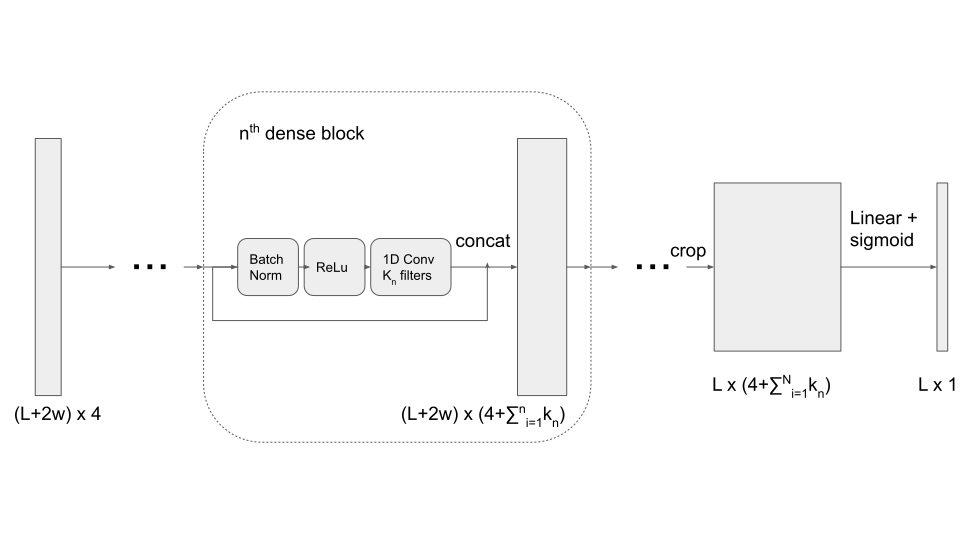
\includegraphics[width=\textwidth]{proposal_dense_net.png}
\caption{Densely connected neural network used for the yeast model}
\label{fig:dense_net}
\centering
\end{figure}

As shown in Fig\ref{fig:dense_net}, to make inference on a stretch of RNA sequence of length $L$,
we need to pad the sequence with $w$ bases on each side. (TODO explanation + how to calculate $w$)
Input consists of the one-hot encoded, padded sequence,
where $A, C, G, U$ bases are encoded as $[1, 0, 0, 0], [0, 1, 0, 0], [0, 0, 1, 0], [0, 0, 0, 1]$, respectively.
The encoded input is then passed through multiple dense blocks,
where each block consists of four components:

\begin{enumerate}
    \item Batch Normalization
    \item ReLu nonlinear activation
    \item 1D Convolution
    \item Concatenation of the block input to the output of convolution
\end{enumerate}

%- {dilation: 1, filter_width: 16, num_filter: 128}
%- {dilation: 2, filter_width: 16, num_filter: 128}
%- {dilation: 4, filter_width: 16, num_filter: 256}
%- {dilation: 8, filter_width: 16, num_filter: 256}
%- {dilation: 16, filter_width: 16, num_filter: 512}

\begin{table}[h!]
    \centering
    \begin{tabular}{||c c c c||}
        \hline
        Block number & Number of filters & Filter width & Dilation rate \\ [0.5ex]
        \hline\hline
        1 & 128 & 16 & 1 \\
        \hline
        2 & 128 & 16 & 2 \\
        \hline
        3 & 256 & 16 & 4 \\
        \hline
        4 & 256 & 16 & 8 \\
        \hline
        5 & 512 & 16 & 16 \\ [1ex]
        \hline
    \end{tabular}
    \caption{Dense block parameters}
    \label{table:conv_layer_params}
\end{table}

We use $5$ dense blocks in this work. The parameter of each layer is as shown in Table\ref{table:conv_layer_params}.
Densely connected block has the advantage that each block receives input from all preceding blocks,
and passes its output to all successive blocks.
The output of the last dense block essentially represents the features learnt from input at multiple resolutions.

The final dense block output is then cropped to account for the input padding,
and then passed through a fully connected layer with sigmoid activation, along the feature dimension.


\section{Training}

%- [chrM, chrVIII, chrII, chrXV]
%- [chrI, chrV, chrXIII, chrIV]
%- [chrVI, chrXI, chrXVI]
%- [chrIII, chrX, chrXII]
%- [chrIX, chrXIV, chrVII]

\begin{table}[h!]
    \centering
    \begin{tabular}{||c c||}
        \hline
        Fold number & Chromosomes \\ [0.5ex]
        \hline\hline
        1 & chrM, chrVIII, chrII, chrXV \\
        \hline
        2 & chrI, chrV, chrXIII, chrIV \\
        \hline
        3 & chrVI, chrXI, chrXVI \\
        \hline
        4 & chrIII, chrX, chrXII \\
        \hline
        5 & chrIX, chrXIV, chrVII \\ [1ex]
        \hline
    \end{tabular}
    \caption{Chromosomes used for each fold}
    \label{table:fold_chrom_split}
\end{table}


We use 5-fold cross validation, where the folds are splited by chromosomes, as shown in Table \ref{table:fold_chrom_split}.

Normalized data points (between $0$ and $1$) are used as soft targets without being converted to binary labels,
and models were trained using a masked cross-entropy loss, as described below.

Due to the nature of DMS modification, G/T bases has no coverage,
thus should be excluded from the calculation of the loss and the gradient.
This is achieve by first computing the per position cross-entropy loss between the prediction and the target,
then multiply it with a binary mask with the same shape as the target array.
Positions with G/T bases are being set to $0$ in the mask, while positions with A/C bases are $1$.
The masked loss are then summed over positions, and minibatch dimension, to calculate the loss for the current minibatch and the gradient for back propagation.

Models were trained using fixed sequence length of $50$ (before padding, sequence length at inference time can be variable),
minibatch size of $10$, Adam optimizer with learning rate $0.0001$ and momentum $0.9$.
To prevent the models from overfitting, L1 and L2 regularizers with weight $0.000001$ was added to the loss,
and training is stopped if validation loss hasn't improved over the last $10$ epochs.

We trained $5$ models, each using one of the folds as validation data, and the rest as training data.


\section{Performance}


\subsection{Cross-validation performance on training dataset}

We first evaluate the model performance on training dataset.
For each transcript, we used the model that wasn't trained on its chromosome to make prediction for all A/C bases.
We computed the Spearman correlation between the prediction and the target for each transcript.
Fig \ref{fig:yeast_cv_performance} shows the distribution of Spearman correlation across all transcripts.

\begin{figure}
\includegraphics[width=\textwidth]{yeast_cv_performance.png}
\caption{Densely connected neural network used for the yeast model}
\label{fig:yeast_cv_performance}
\centering
\end{figure}




\section{Future Work}

TODO RT stop / total coverage

TODO 4 reps, re-weight each position

multi resolution

\chapter{Mouse Model}


\chapter{Human Model}

\chapter{Conclusion and future work}

one dataset that has multiple mods per sequence, so we can reconstruct colleciton of structures

joint learning of accessibility and other data, e.g. chip-seq peaks


\addcontentsline{toc}{chapter}{Bibliography}
\bibliographystyle{plain}
\bibliography{proposal}

\end{document}
